% \documentclass[border=0]{standalone}
\documentclass[a3paper]{article}
\usepackage[left=-2mm,top=2mm,right=0mm,bottom=0mm]{geometry}
\usepackage{tikz}
\usetikzlibrary {backgrounds}
\begin{document}
\thispagestyle{empty}
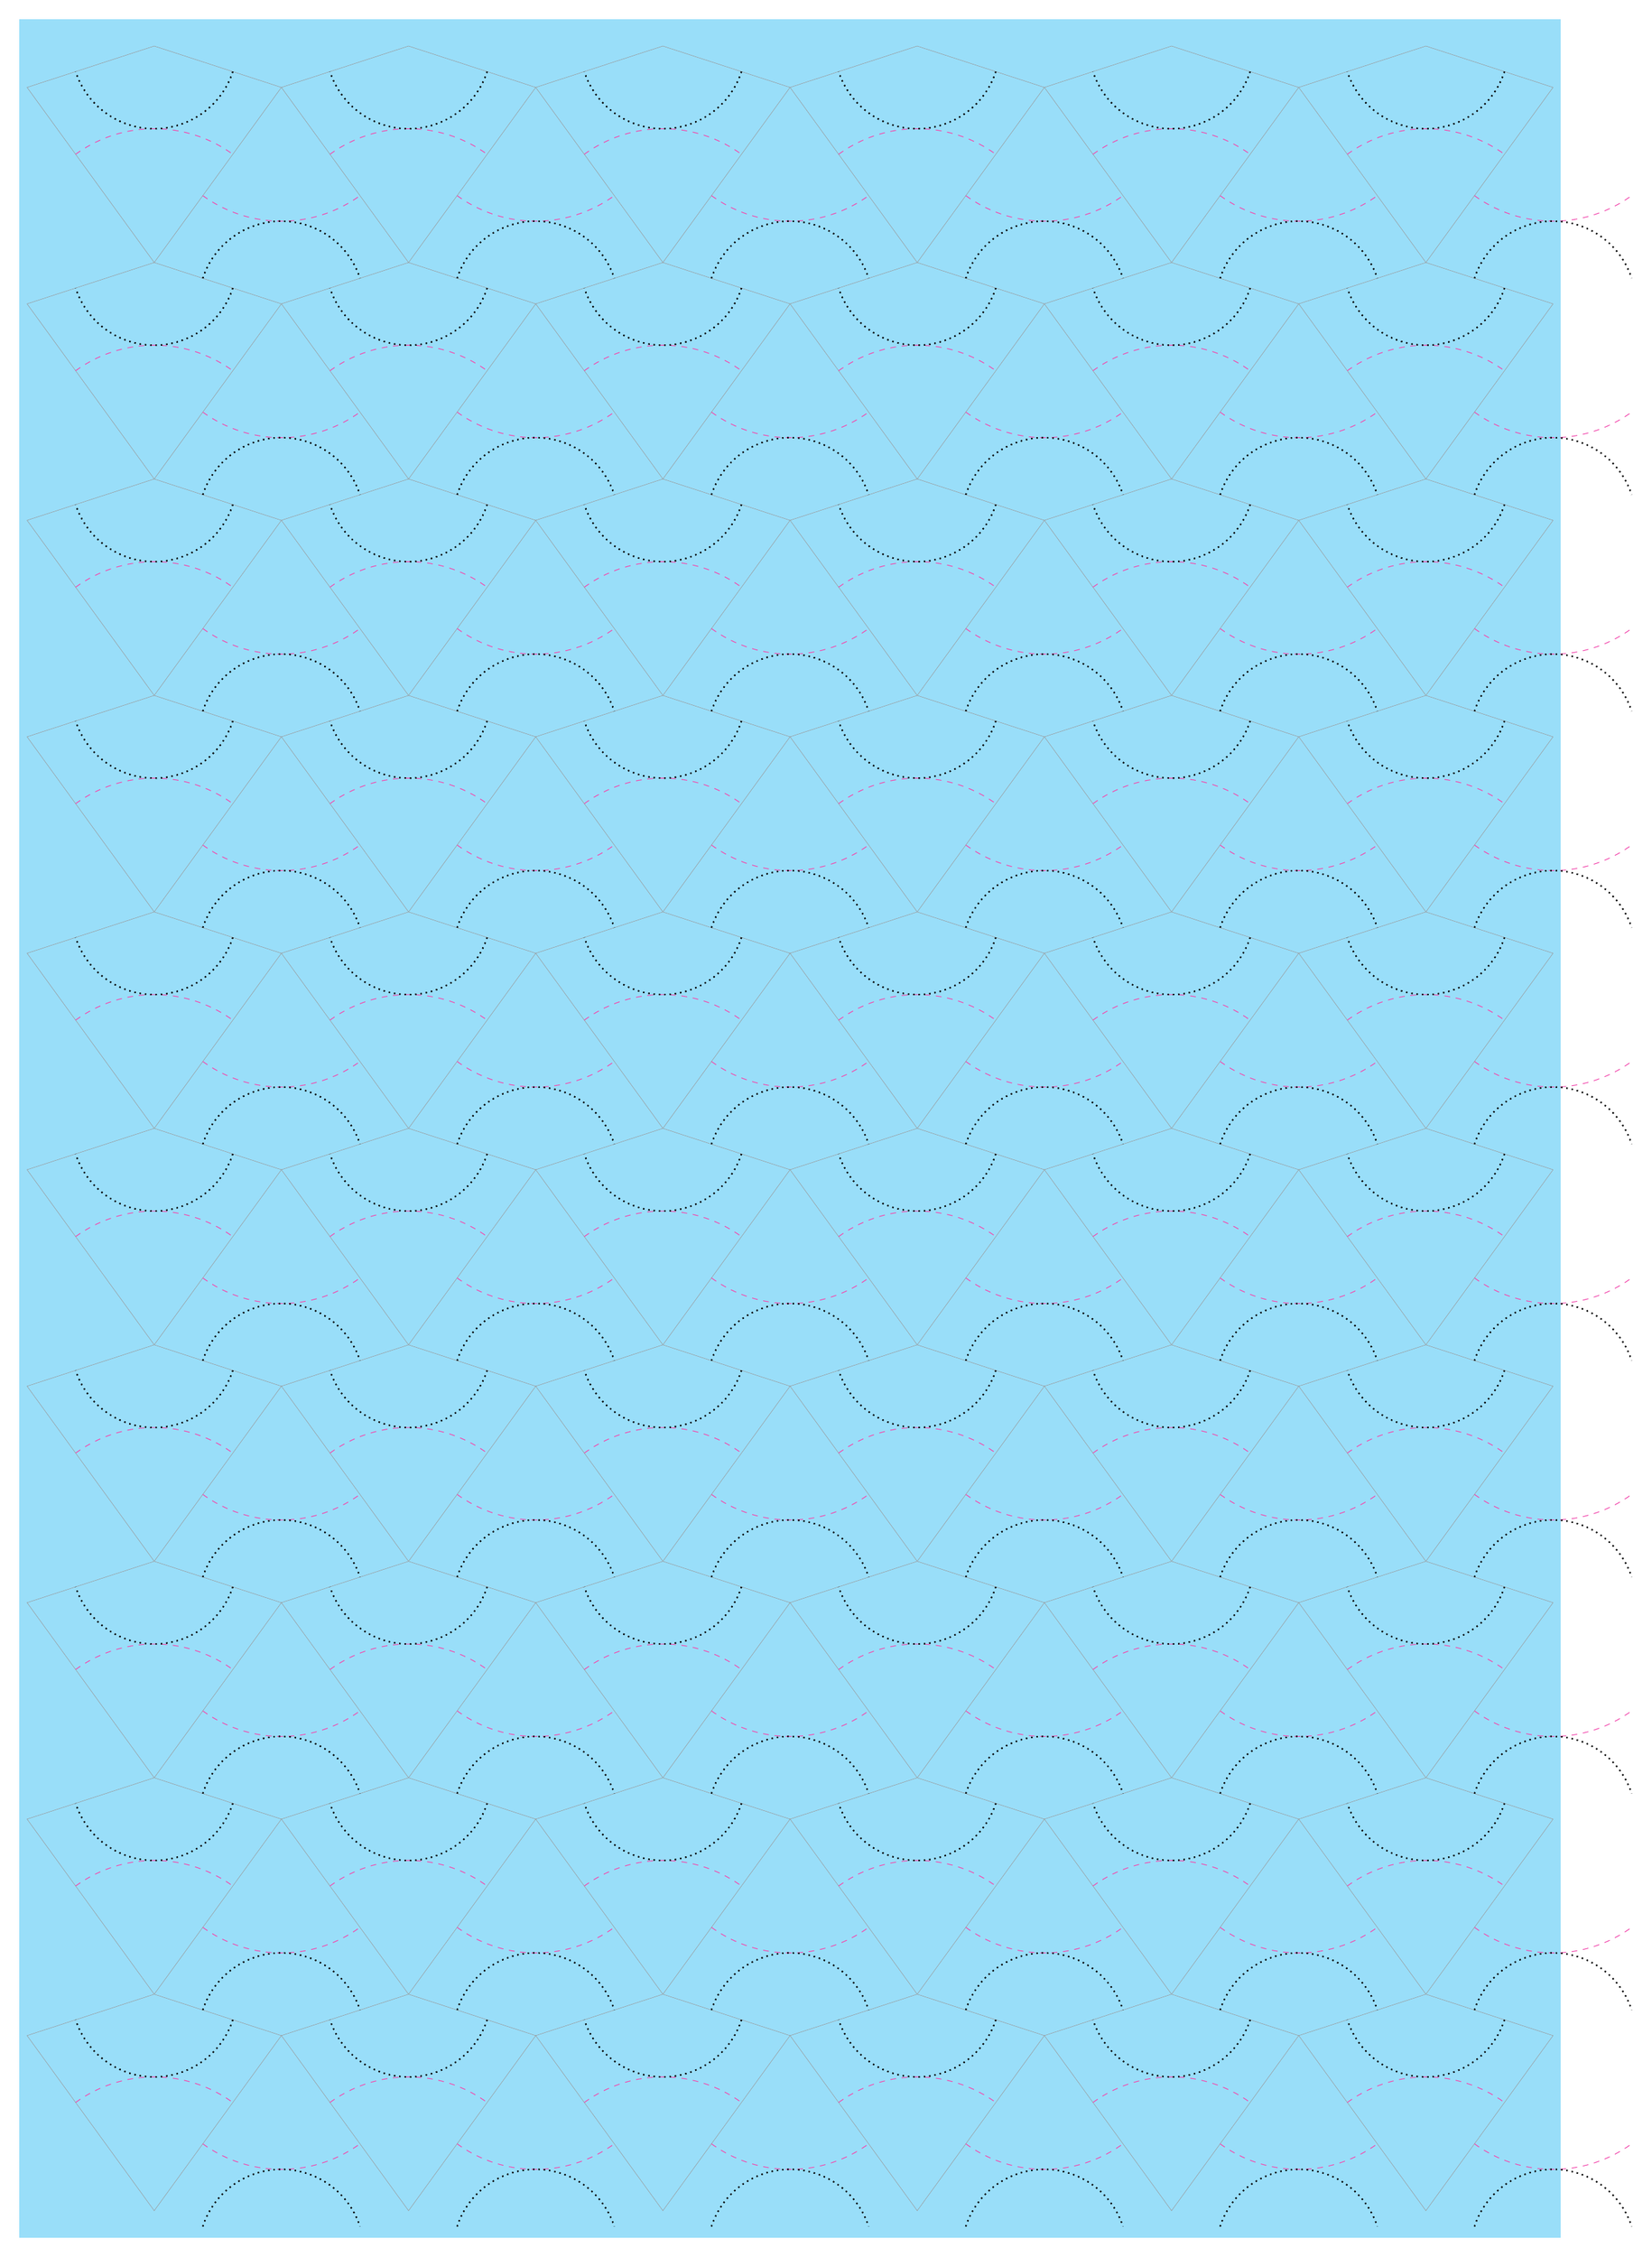
\begin{tikzpicture}
    \begin{scope}[on background layer={color=cyan!40}]
        \fill (-2.5,-.5) rectangle (26,40.5);
        \end{scope}
    \pgfmathsetmacro{\p}{(1+sqrt(5))/2}
    \pgfmathsetmacro{\l}{4}
    \foreach \y in {0,1,2,...,9}{
        \foreach \x in {0,1,...,5}{
            \draw[black!40,very thin] ({(sqrt(3-\p))*\l*\x},{\y*\l}) --++ (54:\l)--++(162:\l/\p)--++(198:\l/\p) -- cycle;
            \draw[dashed,magenta!70] ({(sqrt(3-\p))*\l*\x},{\y*\l})++(126:{\l*\p/(1+\p)}) arc (126:54:{\l*\p/(1+\p)});
            \draw[dashed,magenta!70] ({(sqrt(3-\p))*\l*\x},{\y*\l})++(54:{\l/(1+\p)}) arc (234:306:{\l*\p/(1+\p)});
            \draw[dotted,thick] ({(sqrt(3-\p))*\l*\x},{\y*\l})++(54:\l)++(162:{\l*(\p-1)/(\p+1)}) arc (342:198:{\l/(\p+1)});
            \draw[dotted,thick] ({(sqrt(3-\p))*\l*\x},{\y*\l})++(342:{\l*(\p-1)/(\p+1)}) arc (162:18:{\l/(\p+1)});
        }
    };

\end{tikzpicture}
\end{document}